\documentclass[a4paper,12pt]{article}

\usepackage[utf8x]{inputenc}
\usepackage[T2A]{fontenc}
\usepackage[english, russian]{babel}

% Опционно, требует  apt-get install scalable-cyrfonts.*
% и удаления одной строчки в cyrtimes.sty
% Сточку не удалять!
% \usepackage{cyrtimes}

% Картнки и tikz
\usepackage{graphicx}
\usepackage{tikz}
\usetikzlibrary{snakes,arrows,shapes}


% Некоторая русификация.
\usepackage{misccorr}
\usepackage{indentfirst}
\renewcommand{\labelitemi}{\normalfont\bfseries{--}}

% Увы, поля придётся уменьшить из-за листингов.
\topmargin -1cm
\oddsidemargin -0.5cm
\evensidemargin -0.5cm
\textwidth 17cm
\textheight 24cm

\sloppy

% Оглавление в PDF
\usepackage[
bookmarks=true,
colorlinks=true, linkcolor=black, anchorcolor=black, citecolor=black, menucolor=black,filecolor=black, urlcolor=black,
unicode=true
]{hyperref}

% Для исходного кода в тексте
\newcommand{\Code}[1]{\textbf{#1}}

\usepackage{verbatim}
\usepackage{fancyvrb}
\fvset{frame=leftline, fontsize=\small, framerule=0.4mm, rulecolor=\color{darkgray}, commandchars=\\\{\}}
\renewcommand{\theFancyVerbLine}{\small\arabic{FancyVerbLine}}



\title{Отчёт по лабораторной работе \\ <<IP-маршрутизация>>}
\author{Руднев Дмитрий Николаевич}

\begin{document}

\maketitle

\tableofcontents

% Текст отчёта должен быть читаемым!!! Написанное здесь является рыбой.

\section{Топология сети}

Топология сети и использыемые IP-адреса показаны на рис.~\ref{fig:network}.

\begin{figure}
\centering
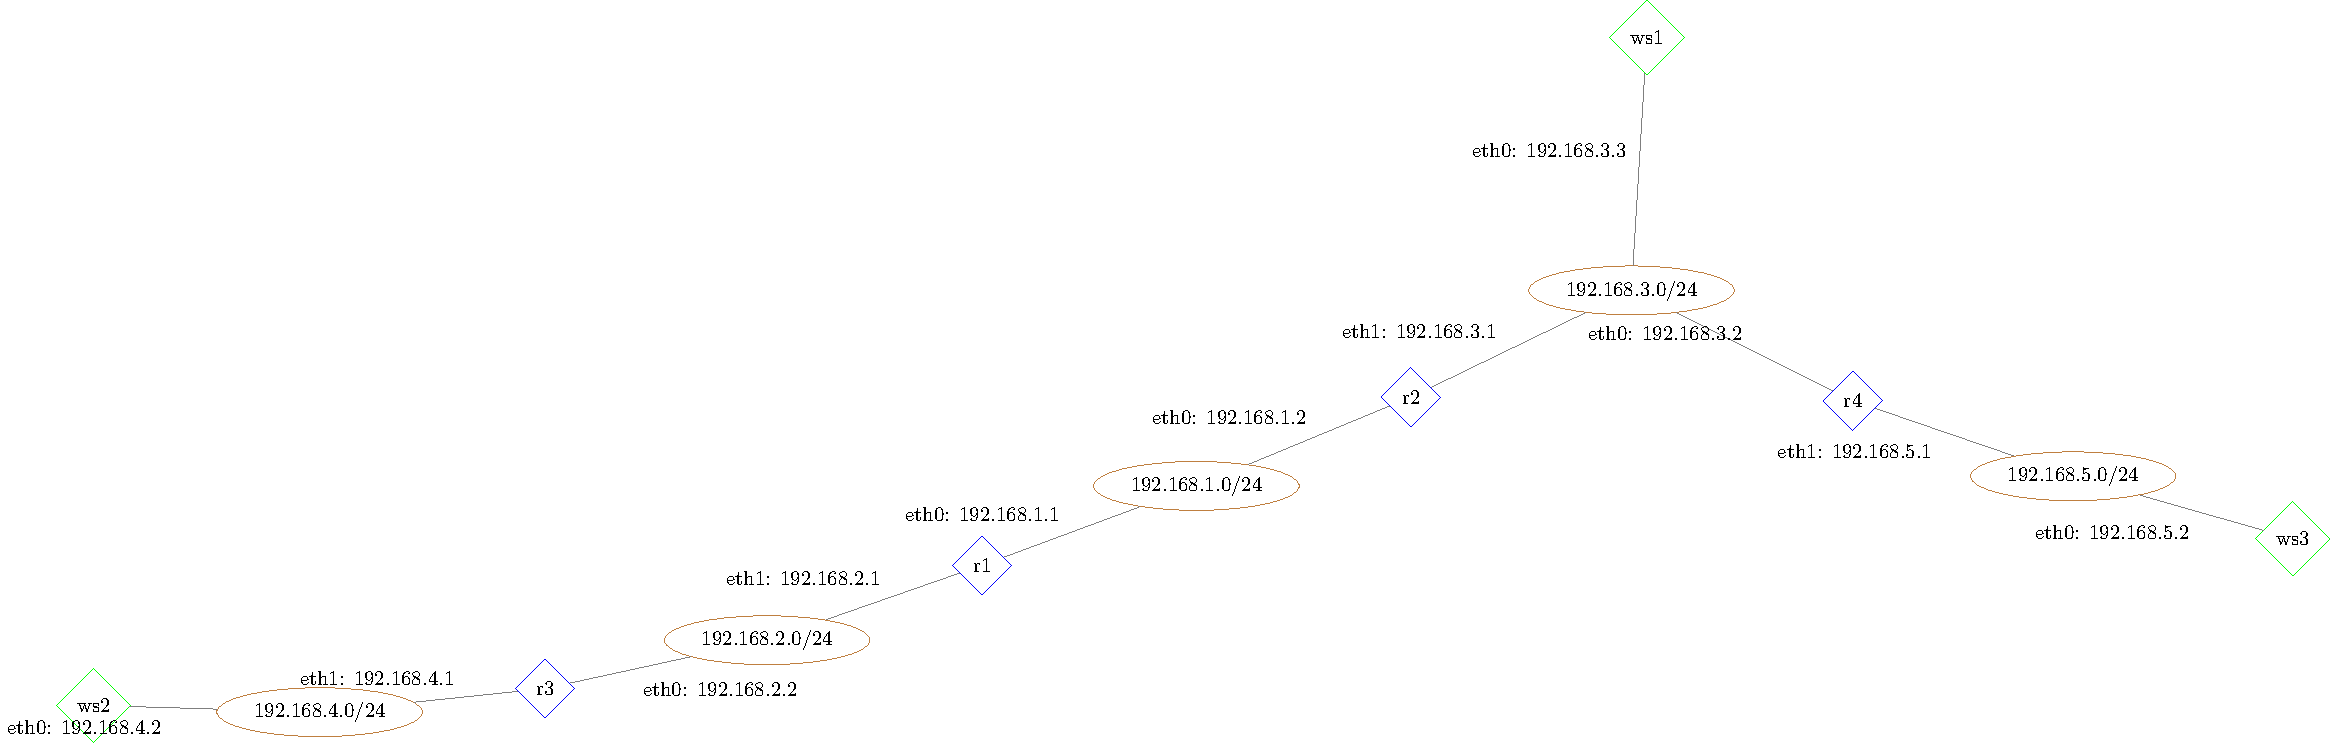
\includegraphics[width=\textwidth]{includes/network_gv.pdf}
\caption{Топология сети}
\label{fig:network}
\end{figure}


\section{Назначение IP-адресов}

Ниже приведён файл настройки протокола IP маршрутизатора r1.

\begin{Verbatim}
auto lo
iface lo inet loopback

auto eth0
iface eth0 inet static
address 192.168.1.1
netmask 255.255.255.0

up ip r add 192.168.3.0/24 via 192.168.1.2 dev eth0
up ip r add 192.168.5.0/24 via 192.168.1.2 dev eth0

down ip r del 192.168.3.0/24
down ip r del 192.168.5.0/24

auto eth1
iface eth1 inet static
address 192.168.2.1
netmask 255.255.255.0

up ip r add 192.168.4.0/24 via 192.168.2.2 dev eth1
down ip r del 192.168.4.0/24
\end{Verbatim}

Ниже приведён файл настройки протокола IP рабочей станции ws1.

\begin{Verbatim}
auto lo
iface lo inet loopback

auto eth0
iface eth0 inet static
address 192.168.3.3
netmask 255.255.255.0
gateway 192.168.3.1
\end{Verbatim}


\section{Таблица маршрутизации}

Вывести (командой ip r) таблицу маршрутизации для \textbf{r1}.

\begin{Verbatim}
192.168.5.0/24 via 192.168.1.2 dev eth0 
192.168.4.0/24 via 192.168.2.2 dev eth1 
192.168.3.0/24 via 192.168.1.2 dev eth0 
192.168.2.0/24 dev eth1  proto kernel  scope link  src 192.168.2.1 
192.168.1.0/24 dev eth0  proto kernel  scope link  src 192.168.1.1 
\end{Verbatim}

Вывести (командой ip r) таблицу маршрутизации для \textbf{r2}.

\begin{Verbatim}
192.168.5.0/24 via 192.168.3.2 dev eth1 
192.168.4.0/24 via 192.168.1.1 dev eth0 
192.168.3.0/24 dev eth1  proto kernel  scope link  src 192.168.3.1 
192.168.2.0/24 via 192.168.1.1 dev eth0 
192.168.1.0/24 dev eth0  proto kernel  scope link  src 192.168.1.2 
\end{Verbatim}

Вывести (командой ip r) таблицу маршрутизации для \textbf{r3}.

\begin{Verbatim}
192.168.5.0/24 via 192.168.2.1 dev eth0 
192.168.4.0/24 dev eth1  proto kernel  scope link  src 192.168.4.1 
192.168.3.0/24 via 192.168.2.1 dev eth0 
192.168.2.0/24 dev eth0  proto kernel  scope link  src 192.168.2.2 
192.168.1.0/24 via 192.168.2.1 dev eth0
\end{Verbatim}

Вывести (командой ip r) таблицу маршрутизации для \textbf{r4}.

\begin{Verbatim}
192.168.5.0/24 dev eth1  proto kernel  scope link  src 192.168.5.1 
192.168.4.0/24 via 192.168.3.1 dev eth0 
192.168.3.0/24 dev eth0  proto kernel  scope link  src 192.168.3.2 
192.168.2.0/24 via 192.168.3.1 dev eth0 
192.168.1.0/24 via 192.168.3.1 dev eth0
\end{Verbatim}

% ... Повторять для всех маршрутизаторов и рабочих станций, где есть что-то кроме gateway.

\section{Проверка настройки сети}

Вывод \textbf{traceroute} от узла ws1 до ws3 при нормальной работе сети.

\begin{Verbatim}
traceroute to 192.168.5.2 (192.168.5.2), 64 hops max, 40 byte packets
 1  192.168.3.1 (192.168.3.1)  2 ms  0 ms  8 ms
 2  192.168.3.2 (192.168.3.2)  19 ms  0 ms  0 ms
 3  192.168.5.2 (192.168.5.2)  6 ms  0 ms  0 ms
\end{Verbatim}

Вывод \textbf{traceroute} от узла ws1 до ws2 при нормальной работе сети.

\begin{Verbatim}
traceroute to 192.168.4.2 (192.168.4.2), 64 hops max, 40 byte packets
 1  192.168.3.1 (192.168.3.1)  0 ms  0 ms  0 ms
 2  192.168.1.1 (192.168.1.1)  12 ms  1 ms  0 ms
 3  192.168.2.2 (192.168.2.2)  11 ms  1 ms  1 ms
 4  192.168.4.2 (192.168.4.2)  12 ms  1 ms  1 ms
\end{Verbatim}

Вывод \textbf{traceroute} от узла ws2 до ws3 при нормальной работе сети.

\begin{Verbatim}
traceroute to 192.168.5.2 (192.168.5.2), 64 hops max, 40 byte packets
 1  192.168.4.1 (192.168.4.1)  1 ms  0 ms  0 ms
 2  192.168.2.1 (192.168.2.1)  0 ms  0 ms  0 ms
 3  192.168.1.2 (192.168.1.2)  0 ms  0 ms  0 ms
 4  192.168.3.2 (192.168.3.2)  11 ms  1 ms  1 ms
 5  192.168.5.2 (192.168.5.2)  1 ms  3 ms  4 ms
\end{Verbatim}


\section{Маршрутизация}

% На пути здесь достаточно быть одному аршрутизатору!

Вначале стоит написать, какие MAC-адреса интерфейсов в опыте были у каких машин.
Затем вывести маршрутную таблицу маршрутизатора (вывод команды ip r!)

\begin{Verbatim}
ws1 eth0 MAC: a6:f9:52:b6:1e:69
ws3 eth0 MAC: b2:0b:69:d6:a7:1e

r2 eth0 MAC: 3a:40:ee:31:9e:cd
r2 eth1 MAC: 12:3e:e2:7d:e3:87
r4 eth0 MAC: 4a:e4:d9:3b:f2:04
r4 eth1 MAC: 42:9b:97:db:b0:a6

маршрутная таблица маршрутизатора r2:
192.168.5.0/24 via 192.168.3.2 dev eth1 
192.168.4.0/24 via 192.168.1.1 dev eth0 
192.168.3.0/24 dev eth1  proto kernel  scope link  src 192.168.3.1 
192.168.2.0/24 via 192.168.1.1 dev eth0 
192.168.1.0/24 dev eth0  proto kernel  scope link  src 192.168.1.2 

маршрутная таблица маршрутизатора r4:
192.168.5.0/24 dev eth1  proto kernel  scope link  src 192.168.5.1 
192.168.4.0/24 via 192.168.3.1 dev eth0 
192.168.3.0/24 dev eth0  proto kernel  scope link  src 192.168.3.2 
192.168.2.0/24 via 192.168.3.1 dev eth0 
192.168.1.0/24 via 192.168.3.1 dev eth0 
\end{Verbatim}

Показаны опыты после стирания кеша ARP.

Далее показана отправка пакета на маршрутизатор (косвенная маршрутизация). 

\begin{Verbatim}
ws1:~# ping -c 1 192.168.5.2
r2 tcpdump:
a6:f9:52:b6:1e:69 > ff:ff:ff:ff:ff:ff, ethertype ARP (0x0806), length 42: arp who-has 192.168.3.1 tell 192.168.3.3
12:3e:e2:7d:e3:87 > a6:f9:52:b6:1e:69, ethertype ARP (0x0806), length 42: arp reply 192.168.3.1 is-at 12:3e:e2:7d:e3:87
a6:f9:52:b6:1e:69 > 12:3e:e2:7d:e3:87, ethertype IPv4 (0x0800), length 98: (tos 0x0, ttl 64, id 0, offset 0, flags [DF], proto ICMP (1), length 84) 192.168.3.3 > 192.168.5.2: ICMP echo request, id 26114, seq 1, length 64
12:3e:e2:7d:e3:87 > ff:ff:ff:ff:ff:ff, ethertype ARP (0x0806), length 42: arp who-has 192.168.3.2 tell 192.168.3.1
4a:e4:d9:3b:f2:04 > 12:3e:e2:7d:e3:87, ethertype ARP (0x0806), length 42: arp reply 192.168.3.2 is-at 4a:e4:d9:3b:f2:04
12:3e:e2:7d:e3:87 > 4a:e4:d9:3b:f2:04, ethertype IPv4 (0x0800), length 98: (tos 0x0, ttl 63, id 0, offset 0, flags [DF], proto ICMP (1), length 84) 192.168.3.3 > 192.168.5.2: ICMP echo request, id 26114, seq 1, length 64

\end{Verbatim}

Затем маршрутизатор отправил его далее.

\begin{Verbatim}
r2 tcpdump:
12:3e:e2:7d:e3:87 > 4a:e4:d9:3b:f2:04, ethertype IPv4 (0x0800), length 98: (tos 0x0, ttl 63, id 0, offset 0, flags [DF], proto ICMP (1), length 84) 192.168.3.3 > 192.168.5.2: ICMP echo request, id 26114, seq 1, length 64

r4 tcpdump:
a6:f9:52:b6:1e:69 > ff:ff:ff:ff:ff:ff, ethertype ARP (0x0806), length 42: arp who-has 192.168.3.1 tell 192.168.3.3
12:3e:e2:7d:e3:87 > ff:ff:ff:ff:ff:ff, ethertype ARP (0x0806), length 42: arp who-has 192.168.3.2 tell 192.168.3.1
4a:e4:d9:3b:f2:04 > 12:3e:e2:7d:e3:87, ethertype ARP (0x0806), length 42: arp reply 192.168.3.2 is-at 4a:e4:d9:3b:f2:04
12:3e:e2:7d:e3:87 > 4a:e4:d9:3b:f2:04, ethertype IPv4 (0x0800), length 98: (tos 0x0, ttl 63, id 0, offset 0, flags [DF], proto ICMP (1), length 84) 192.168.3.3 > 192.168.5.2: ICMP echo request, id 26114, seq 1, length 64

ws3 tcpdump:
42:9b:97:db:b0:a6 > ff:ff:ff:ff:ff:ff, ethertype ARP (0x0806), length 42: arp who-has 192.168.5.2 tell 192.168.5.1
b2:0b:69:d6:a7:1e > 42:9b:97:db:b0:a6, ethertype ARP (0x0806), length 42: arp reply 192.168.5.2 is-at b2:0b:69:d6:a7:1e
42:9b:97:db:b0:a6 > b2:0b:69:d6:a7:1e, ethertype IPv4 (0x0800), length 98: (tos 0x0, ttl 62, id 0, offset 0, flags [DF], proto ICMP (1), length 84) 192.168.3.3 > 192.168.5.2: ICMP echo request, id 26114, seq 1, length 64
b2:0b:69:d6:a7:1e > 42:9b:97:db:b0:a6, ethertype IPv4 (0x0800), length 98: (tos 0x0, ttl 64, id 25129, offset 0, flags [none], proto ICMP (1), length 84) 192.168.5.2 > 192.168.3.3: ICMP echo reply, id 26114, seq 1, length 64
\end{Verbatim}

\section{Продолжительность жизни пакета}

Сначала написать как и на чём ломали. 

\begin{Verbatim}
r1 router:
ip l set eth1 down
ip r add 192.168.4.0/24 via 192.168.1.2 dev eth0
\end{Verbatim}

Потом какая-то таблица вышла.

\begin{Verbatim}
192.168.5.0/24 via 192.168.1.2 dev eth0 
192.168.4.0/24 via 192.168.1.2 dev eth0 
192.168.3.0/24 via 192.168.1.2 dev eth0 
192.168.1.0/24 dev eth0  proto kernel  scope link  src 192.168.1.1
\end{Verbatim}

Потом что слали.

\begin{Verbatim}
ws1:~# ping -c 1 192.168.4.2
\end{Verbatim}

И что в итоге получилось.

\begin{Verbatim}
r1 tcpdump:
3a:40:ee:31:9e:cd > 0e:ab:f8:0c:10:4b, ethertype IPv4 (0x0800), length 98: (tos 0x0, ttl 63, id 0, offset 0, flags [DF], proto ICMP (1), length 84) 192.168.3.3 > 192.168.4.2: ICMP echo request, id 26882, seq 1, length 64
0e:ab:f8:0c:10:4b > 3a:40:ee:31:9e:cd, ethertype IPv4 (0x0800), length 98: (tos 0x0, ttl 62, id 0, offset 0, flags [DF], proto ICMP (1), length 84) 192.168.3.3 > 192.168.4.2: ICMP echo request, id 26882, seq 1, length 64
3a:40:ee:31:9e:cd > 0e:ab:f8:0c:10:4b, ethertype IPv4 (0x0800), length 98: (tos 0x0, ttl 61, id 0, offset 0, flags [DF], proto ICMP (1), length 84) 192.168.3.3 > 192.168.4.2: ICMP echo request, id 26882, seq 1, length 64
...
0e:ab:f8:0c:10:4b > 3a:40:ee:31:9e:cd, ethertype IPv4 (0x0800), length 126: (tos 0xc0, ttl 64, id 64449, offset 0, flags [none], proto ICMP (1), length 112) 192.168.1.1 > 192.168.3.3: ICMP time exceeded in-transit, length 92
	(tos 0x0, ttl 1, id 0, offset 0, flags [DF], proto ICMP (1), length 84) 192.168.3.3 > 192.168.4.2: ICMP echo request, id 26882, seq 1, length 64
\end{Verbatim}

И r1 в итоге отравил сообщение о завершении жизни.

\section{Изучение IP-фрагментации}

Написать, на каких узлах и как изменяли MTU.


\begin{Verbatim}
r1:
 ip l set dev eth0 mtu 576
\end{Verbatim}

\begin{Verbatim}
r2:
 ip l set dev eth0 mtu 576
\end{Verbatim}

% Напоминаем, что PMTU следует отключить!

Какие команды давали для тестирования и где.

\begin{Verbatim}
ws1:
ping -c 1 -s 1000 192.168.4.2
\end{Verbatim}

Вывод \textbf{tcpdump} на маршрутизаторе перед сетью с уменьшенным MTU.

% Вывод в ширину можно и сократить, удалив несущественные моменты!

\begin{Verbatim}
r2 eth0:
IP (tos 0x0, ttl 63, id 55859, offset 0, flags [+], proto ICMP (1), length 572) 192.168.3.3 > 192.168.4.2: ICMP echo request, id 27650, seq 1, length 552
IP (tos 0x0, ttl 63, id 55859, offset 552, flags [none], proto ICMP (1), length 476) 192.168.3.3 > 192.168.4.2: icmp
\end{Verbatim}

Вывод \textbf{tcpdump} на маршрутизаторе после сети с уменьшенным MTU.

% Вывод в ширину можно и сократить, удалив несущественные моменты!

\begin{Verbatim}
r1 eth0:
IP (tos 0x0, ttl 63, id 55859, offset 0, flags [+], proto ICMP (1), length 572) 192.168.3.3 > 192.168.4.2: ICMP echo request, id 27650, seq 1, length 552
IP (tos 0x0, ttl 63, id 55859, offset 552, flags [none], proto ICMP (1), length 476) 192.168.3.3 > 192.168.4.2: icmp
r1 eth1:
IP (tos 0x0, ttl 62, id 55861, offset 0, flags [none], proto ICMP (1), length 1028) 192.168.3.3 > 192.168.4.2: ICMP echo request, id 28162, seq 1, length 1008
\end{Verbatim}


Вывод \textbf{tcpdump} на узле получателя.

\begin{Verbatim}
ws2:
IP (tos 0x0, ttl 61, id 55860, offset 0, flags [none], proto ICMP (1), length 1028) 192.168.3.3 > 192.168.4.2: ICMP echo request, id 27906, seq 1, length 1008
\end{Verbatim}


\section{Отсутствие сети}

Аналогично опишите опыт, когда маршрутизатор отсылает сообщение об отстутствии с сети.
С командами и выводом, мак адреса не нужны.
\begin{Verbatim}
ws1:
ping -c 1 -s 1000 10.10.4.2
r2:
IP (...) 192.168.3.1 > 192.168.3.3: ICMP net 10.10.4.2 unreachable, length 556
	IP (...) 192.168.3.3 > 10.10.4.2: ICMP echo request, id 28418, seq 1, length 1008[|icmp]
\end{Verbatim}

\section{Отсутствие IP-адреса в сети}

Аналогично опишите опыт, когда маршрутизатор отсылает сообщение об отстутствии требуемого IP-адреса в сети.
С командами и выводом, мак адреса не нужны.

\begin{Verbatim}
ws1:
ping -c 1 -s 1000 192.168.4.100
r3:
IP (...) 192.168.2.2 > 192.168.3.3: ICMP host 192.168.4.100 unreachable, length 556
	IP (...) 192.168.3.3 > 192.168.4.100: ICMP echo request, id 28674, seq 1, length 1008[|icmp]
\end{Verbatim}

\end{document}
